\section{Compressed Sensing with Coordinate Descent}\label{cd}
The idea behind compressed sensing is we use prior information about the image, and find the most likely image $x$ from all possible solutions. In practice, we formulate a minimization problem with a data and regularization term. The data term forces the image to be as close to the measured Visibilities as possible, and the regularization term tells us how likely the image is to be true. 

The regularization is responsible for an accurate reconstruction. In this work, two regularizations are used. The L1 pixel regularization is used to demonstrate a simple version of the coordinate descent algorithm. For the actual algorithm starlet regularization is used. Starlets have been used as regularization for the LOFAR interferometer\cite{girard2015sparse}, which has been shown to work.

First, let us look at the coordinate descent algorithm in its simplest form, and discuss its properties. we want to minimize the objective \eqref{cd:clean}, where the data term $\left \| V - F^{-1}x \right \|_2^2$ forces the image to be close to the Visibilities $V$, and the regularization term $\left \| x \right \|_1$ forces the image to have as few non-zero pixels as possible. The parameter $\lambda$ represents our trade-off between reconstruction accuracy and regularization. 
 
\begin{equation}\label{cd:clean}
	\underset{x}{minimize} \: \left \| V - F^{-1}x \right \|_2^2 + \lambda \left \| x \right \|_1 \\
\end{equation}

The objective function \eqref{cd:clean} has a property, which we can exploit with Coordinate Descent: The optimum for a single pixel, if we keep all others fixed, turns out to be a parabola. The optimum for a single pixel of \eqref{cd:clean} is simply finding the apex of a parabola, followed by a shrink operation\footnote{The shrink operation reduces the magnitude of the pixel by $\lambda$. For example: Pixel $x = -12.4$, $\lambda = 0.6$. The new pixel value after shrinkage follows as $shrink(-12.4, 0.6) = -11.9$}. Sadly, the pixels are not independent of each other, and we need multiple iterations over all pixels to converge. This leads to the following reconstruction algorithm, written in python code:

\begin{lstlisting} 
def coordinate_descent(V_residual, x, lambda, max_iter):
	for k in range(0, max_iter):
		for i in pixels_row:
			for j in pixels_column:
				x_old = x[i, j]
				fourier_column = calculate_fourier_transform(i, j)
				fr = real(fourier_column)
				fi = imag(fourier_column)
				rr = real(V_residual)
				ri = imag(V_residual)
				
				#find apex
				a = sum(fr**2 + 2*fr*fi + fi**2)
				b = sum(fr*rr + fr*ri + fi*rr + fi*ri)
				x_new = b / a + x_old
				
				x_new = shrink(x_new, lambda)
				x[i, j] = x_new
				V_residual = V_residual - fourier_column * (x_new - x_old)
\end{lstlisting}\label{cd:basic}

The simple version of coordinate descent converges to a solution which is similar to CLEAN. The convergence rate of coordinate descent is not well understood. Our image reconstruction problem falls in the class of quadratic programming, in coordinate descent converges at least linearly\cite{luo1992convergence}. In practice, the convergence rate can be sped up with heuristics like active set\cite{activeset} and $\lambda$\cite{lambda}. Furthermore, coordinate descent is robust, even when the residual vector is only approximated, which is useful for distributing the algorithm.

The simple approach calculates the whole Fourier Transform Matrix $F^{-1}$ explicitly. The upside is that we do an exact $w$-term correction. The downside is $F^{-1}$ is too large to keep in memory, and too expensive to calculate on the fly for the scale of MeerKAT reconstructions. 

The starlet transform is used from here on. Instead of reconstructing the image directly, we represent the image as a combination of starlets $x = D\alpha$. Where $D$ is an over-complete dictionary of starlets, and $\alpha$ is the starlet component vector. Since the dictionary $D$ is over-complete, it is a matrix with more columns than rows, and does generally not have an inverse (more formally:$D^{-1}x \neq \alpha$). However, the starlet transform does have an pseudo-inverse. In this work, the pseudo inverse is used to only look at a subset of starlet components which are likely to be non-zero, and only evaluate a subset of columns of $F^{-1}$ .

\subsection{Starlet Transform} \label{cd:starlets}

\begin{figure}[h]
	\centering
	\begin{subfigure}[b]{0.4\linewidth}
		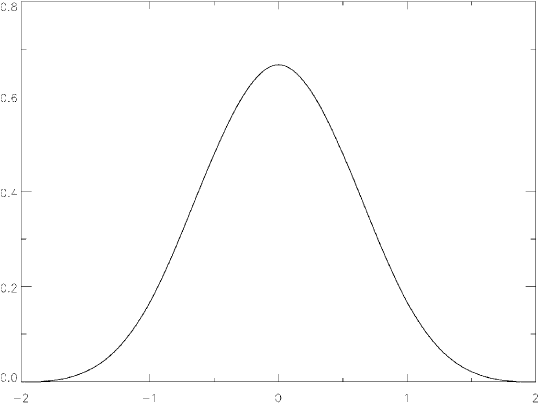
\includegraphics[width=\linewidth]{./chapters/05.algorithms/starlets/scaling.png}
		\caption{Spline scaling function}
		\label{cd:starlets:scaling}
	\end{subfigure}
	\begin{subfigure}[b]{0.4\linewidth}
		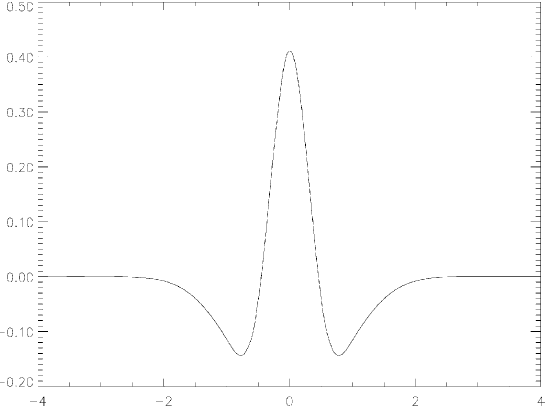
\includegraphics[width=\linewidth]{./chapters/05.algorithms/starlets/wavelet.png}
		\caption{Wavelet function}
		\label{cd:starlets:wavelet}
	\end{subfigure}
	\caption{Scaling and wavelet function of the starlet wavelet. Source: \cite{starck2015starlet}}
	\label{cd:starlets:figure}
\end{figure}

The starlet transform is an Isotropic Undecimated Wavelet Transform (IUWT) based on the starlet wavelet shown in figure \ref{cd:starlets:figure}. The IUWT decomposes an image into multiple layers, each representing parts of the image at different scales. The lower layers contain small structures like point sources, while the higher layers contain extended emissions like hydrogen clouds. The two transforms are shown in equation \eqref{cd:starlet:backwards} and \eqref{cd:starlet:decomposition}. The transformation from starlets to image $x$, shown in \eqref{cd:starlet:backwards}, is a simple addition of all $J$ layers. The transformation from image $x$ to starlet space, shown in \eqref{cd:starlet:decomposition} is done with a multi-scale wavelet decomposition.

\begin{equation} \label{cd:starlet:backwards}
\bm{x} = \bm{w_0} + \bm{w_1} + \ldots + \bm{w_{J-1}} + \bm{c_J}
\end{equation}

\begin{equation}\label{cd:starlet:decomposition}
	\begin{split}
		c_0 &= \bm{x} \star S_0 \\
		\bm{w_0} &= \bm{x} - c_0
	\end{split}
	\qquad
	\begin{split}
		c_1 &= c_0 \star S_1 \\
		\bm{w_1} &= c_0 - c_1
	\end{split}
	\qquad \ldots \qquad
	\begin{split}
		c_{J-1} &= c_{J-2} \star S_{J-1} \\
		\bm{w_{J-1}} &= c_{J-2} - c_{J-1}
	\end{split}
	\qquad
	\begin{split}
		\bm{c_J} &= c_{J-1} \star S_J
	\end{split}
\end{equation}

Let us look at the multi-scale wavelet decomposition in more detail. $w_i$ represents the starlet components at layer $i$, where $w_0$ contains the smallest structures in the image, and $w_{J-1}$ contains the largest structures. Note that the starlets $w_i$, $c_i$ and the image $x$ all have the same dimensions. $c_i$ contains an ever increasingly blurred version of the image $x$. $c_i$ represents the image convolved with all the scaling functions $S_0, S_1, \ldots, S_i$, where $S_i$ is the scaling function shown in figure \ref{cd:starlets:scaling} of the layer $i$. The scaling function increases in size for each successive layer. 

The decomposition starts iteratively, blurrs the image $x$ with the smallest scaling function $S_0$. 


The last, heavily blurred $c_J$ contains the structures which were too big to represent with the largest starlets, and is the last layer of the decomposition.

This is an over-complete representation. Many different components can explain the same pixel.




\subsection{Active set heuristic with Starlets}\label{cd:heuristic}

The multi-scale decomposition can be used to estimate the which starlet components $w_i$ are likely to be non-zero. The figure \ref{cd:heuristic:figure} shows an example of the process. Each "pixel" in \ref{cd:heuristic:starlet} represents a starlet at scale 0, i.e. point sources. We can apply the shrink operator on the $w_0$ map, is essentially a parameter estimation. This property is used in the SASIR\cite{girard2015sparse} reconstruction, which uses the Fast Iterative Shrinkage-Thresholding Algorithm (FISTA) for optimization.

\begin{figure}[h]
	\centering
	\begin{subfigure}[b]{0.45\linewidth}
		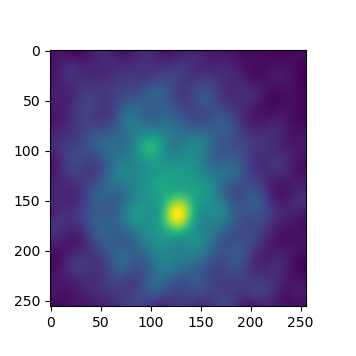
\includegraphics[width=\linewidth]{./chapters/05.algorithms/sim02/sim02_point_dirty.png}
		\caption{Dirty Image with two point sources.}
		\label{cd:heuristic:dirty}
	\end{subfigure}
	\begin{subfigure}[b]{0.45\linewidth}
		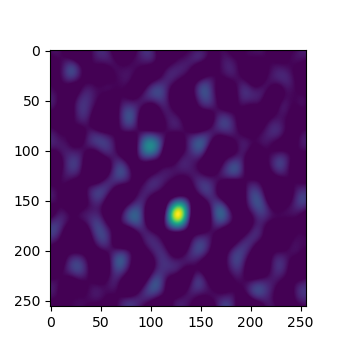
\includegraphics[width=\linewidth]{./chapters/05.algorithms/sim02/starlets0.png}
		\caption{Layer $w_0$ of the multi-scale decomposition.}
		\label{cd:heuristic:starlet}
	\end{subfigure}
	\caption{Dirty map and $w_0$ starlet layer. The right image shows the probability distribution for point sources in the dirty image.}
	\label{cd:heuristic:figure}
\end{figure}

For our purposes, we use the result of the decomposition as a probability distribution. The higher the values of the decomposed $w_i$, the more likely it is to be non-zero.

the X highest values of the $w_i$ decomposition are put into the active set. Only components in the active set get optimized.

Note however that the different locations are dependent on each other. The image \ref{cd:heuristic:starlet} shows two areas for the two point sources. From the $w_0$ map alone it is hard to know if the center blob is due to a single point source, or multiple point sources in a small area.


\subsection{Coordinate Descent Implementation}
Proof of concept implementation. There are many ways to improve the efficiency and the convergence speed. It is here to show  the general if it is possible of the approach and if we can truly only calculate a subset of $F^{-1}$ columns.

The objective function \eqref{cd:starlet} minimizes the starlet components $\alpha$. This objective leads again to a parabola in the one dimensional case, and we can analytically find the optimum for a single component when all others are fixed. 

\begin{equation}\label{cd:starlet}
\underset{\alpha}{minimize} \: \left \| V - F^{-1}D\alpha \right \|_2^2 + \lambda \left \| \alpha \right \|_1 \\
\end{equation}

There are still a few problems to solve, like how to handle the matrix product $F^{-1}D$, 

How to iterate over the image in detail.



\subsubsection{Handling the Matrix Product $F^{-1}D$}
With the active set heuristic, we iterate over a limited number of starlet components at a time. The question remains, how the matrix product $F^{-1}D$ can be calculated efficiently. Since starlet transform is just made up of a couple of deconvolutions, we do not have to calculate the product $F^{-1}D$ explicitly. 

$w_2 = (F^{-2}V \star S_0 \star S_1) - (F^{-2}V \star S_0 \star S_1 \star S_2)$.

Convolution in image space is a multiplication in Visibility space. This means if we replace $x$ with the Visibilities $V$ and Fourier transform the kernel $FS_i = \hat{S_i}$ the rest, we $w_2 = F^{-1}V(\hat{S_0}\hat{S_1} - \hat{S_0}\hat{S_1}\hat{S_2}) $ which simplifies into 
We can pre-calculate the convolutions for each layer $C_{w_2} = (\hat{S_0}\hat{S_1} - \hat{S_0}\hat{S_1}\hat{S_2})$

How many layers are needed. starlets rise in pixels with $2^J$. Meaning if we want starlets over the whole image, the number of starlets rise logarithmically to the image dimensions.

\subsubsection{Iteration scheme}
Many ways to iterate over the image

\begin{lstlisting} 
def coordinate_descent(V_residual, x, lambda, max_iter):
	for k in range(0, max_iter):
		for i in pixels_row:
			for j in pixels_column:
				x_old = x[i, j]
				fourier_column = calculate_fourier_transform(i, j)
				fr = real(fourier_column)
				fi = imag(fourier_column)
				rr = real(V_residual)
				ri = imag(V_residual)
				
				#find apex
				a = sum(fr**2 + 2*fr*fi + fi**2)
				b = sum(fr*rr + fr*ri + fi*rr + fi*ri)
				x_new = b / a + x_old
				
				x_new = shrink(x_new, lambda)
				x[i, j] = x_new
				V_residual = V_residual - fourier_column * (x_new - x_old)
\end{lstlisting}\label{cd:implementation}

coordinate descent with active set heuristic

\subsubsection{Non-uniform FFT approximations}
Non uniform FFT to calculate the convolution KERNELS!!


Stupid approach with line search. Could be done more efficiently by using the histogram of the starlet level.

